\documentclass{slides}
\usepackage[british]{babel}
\usepackage[utf8]{inputenc}
\usepackage[T1]{fontenc}
\usepackage{csquotes}
\usepackage[style=apa, sortcites=true, sorting=nyt,backend=biber]{biblatex}
\DeclareLanguageMapping{british}{british-apa}
\addbibresource{references.bib}
\usepackage{framed, color}
\definecolor{shadecolor}{rgb}{1,0.8,0.3}
\usepackage{soul}
\newcommand{\mathcolorbox}[2]{\colorbox{#1}{$\displaystyle #2$}}

\graphicspath{{./gfx/}}
% Frame number
\setbeamertemplate{footline}[frame number]

\title[]{ No scope for planning -- language pre-planning as mixture process }

\author{\small Jens Roeser \\ $\phantom{foo}$ \\ Mark Torrance $\phantom{foo}$ Mark Andrews $\phantom{foo}$ Thom Baguley \\$\phantom{foo}$ \\ Nottingham Trent University, UK \\ \url{jens.roeser@ntu.ac.uk} }

\institute{26th AMLaP, University of Potsdam}
\date{Sept 3, 2020}

\begin{document}\frame{\titlepage}

	\begin{frame}{Turning ideas into language \parencite{bock1994}}

\begin{minipage}[t]{.45\textwidth}
\begin{small}
\begin{itemize}
	\item Message units are unordered.
	\item Output requires linearisation of words. % of a hierarchically structured linguistic plan.
	\item Linearisation is subject to pragmatic, lexical and / or syntactic factors. 
\end{itemize}
\end{small}
\end{minipage}

\begin{backgroundblock}{60mm}{20mm}	
	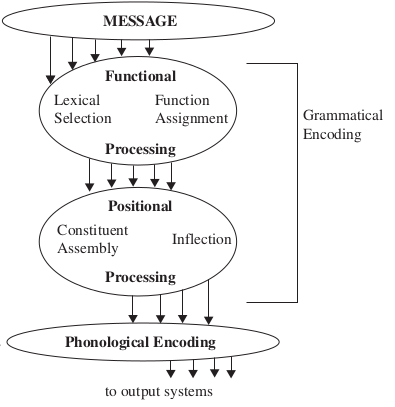
\includegraphics[scale=.45]{gfx/BLmodel.png}
\end{backgroundblock}

\end{frame}

\begin{frame}
	\begin{Large}
		\begin{center}
			\textit{To what extent does syntax affect the linearisation of the output?}
		\end{center}
	\end{Large}
\end{frame}


\begin{frame}{\only<1,5,10-13>{Syntax in language production \parencite{bock2014syntactically}}}

% P 25 in Bock and Ferreira 2014: Paul (1886/190) and Wundt (1912)
% Paul: incremental lexical view
% Wundt: aboutness relations at the core
% Kuchinski relational vs non-relational 

\only<1,5,10-13>{
\begin{small}
	\begin{enumerate}
	\item \uncover<1->{Syntax is an emergent property of lexically-driven planning.}
	\item \uncover<5->{Syntactic relations guide lexical retrieval.}
	\begin{itemize}
		\item[a.] \uncover<10->{\textbf{Deterministic:} syntax determines size of planning unit.}
		\item[b.] \uncover<11->{\textbf{Non-deterministic:} multiple candidate structures   \parencite{kempen1987incremental}.}		
	\end{itemize}
	\item \uncover<12->{Either route (relational and non-relational) is available \parencite[at the message level; see][]{konopka2014priming}.}
	\end{enumerate}
\end{small}

\vspace{1cm}
\begin{center}
	\uncover<13->{\textit{Consider the following evidence for possibility (2a).}}
\end{center}
}

\begin{backgroundblock}{10mm}{10mm}	
	\only<2,3,4>{
	\begin{tikzpicture}
		\node[anchor=north west,rectangle, draw, thick, rounded corners, draw=black, inner sep=3.5pt] (screen) at (0,0) {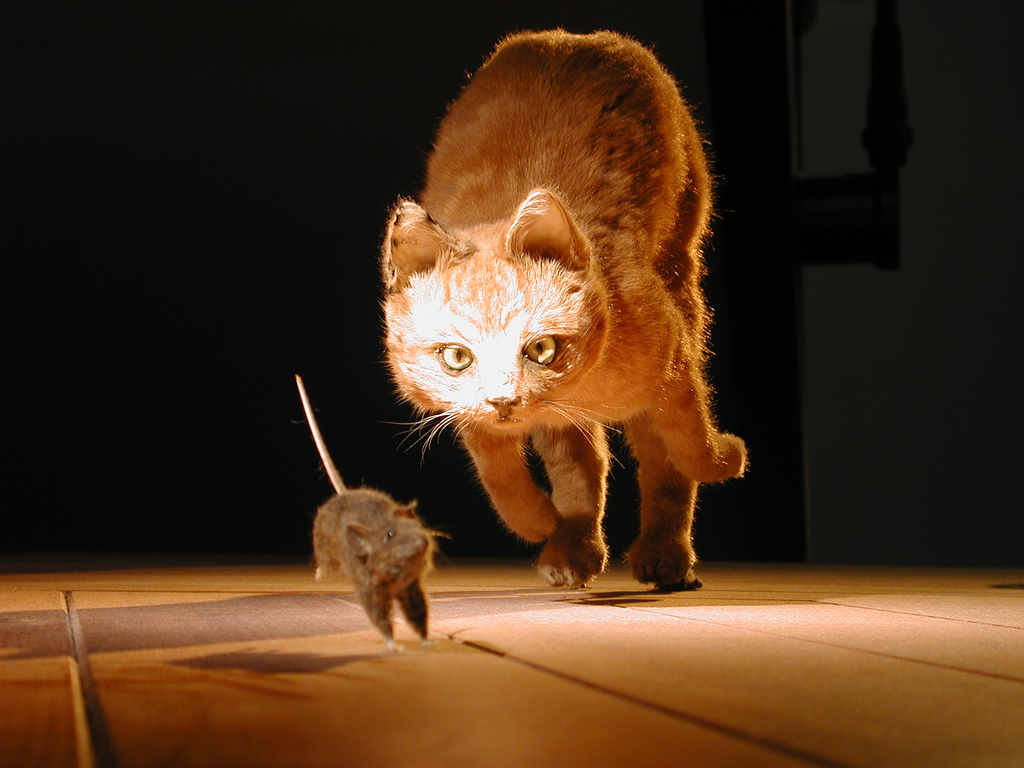
\includegraphics[scale=.1]{gfx/cat2.jpg}};
		
		%% CHUNK 1
		\only<2->{\node[below left = 1cm of screen, rectangle, draw, fill=gray!20!white] (message) {Message};}
		\only<2->{\node[below right = .25cm and 0cm of message, rectangle, draw, fill=gray!40!white, color=gray!40!white] (message2) {Message};}
		\only<2->{\draw[red!60!black, thick] (2.1,-1.2) circle (1cm);}
		\only<2->{\draw[->, thick] (0.9,-1.7) -- (message);}
		\only<2->{\node[below = .25cm of message2, rectangle, draw] (lemma) {CAT};}
		\only<2->{\draw[->, dashed, thick, to path={|- (\tikztotarget)}] (message) edge (message2);}
		
		%% CHUNK 2
		\only<3->{\node[right = .25cm of message, rectangle, draw, fill=gray!20!white, color=gray!20!white] (messageU2) {Message};}	
		\only<3->{\draw[->, thick] (1.2,-2) -- (messageU2);}
		\only<3->{\node[right = .25cm of message2, rectangle, draw, fill=gray!40!white, color=gray!40!white] (messageL2) {Message};}
		\only<3->{\draw[->, dashed, thick, to path={|- (\tikztotarget)}] (messageU2) edge (messageL2);}
		\only<3->{\node[below = .25cm of messageL2, rectangle, draw] (lemma2) {CHASING};}
		
		%% CHUNK 3
		\only<4->{\node[right = .25cm of messageU2, rectangle, draw, fill=gray!20!white, color=gray!20!white] (messageU3) {Message};}	
		\only<4->{\draw[->, thick] (1.5,-2) -- (messageU3);}
		\only<4->{\node[right = .25cm of messageL2, rectangle, draw, fill=gray!40!white, color=gray!40!white] (messageL3) {Message};}
		\only<4->{\draw[->, dashed, thick, to path={|- (\tikztotarget)}] (messageU3) edge (messageL3);}
		\only<4->{\node[below = .25cm of messageL3, rectangle, draw] (lemma3) {RAT};}
		
		
	\end{tikzpicture}
	}
	\only<6-9>{
	\begin{tikzpicture}
		\node[anchor=north west,rectangle, draw, thick, rounded corners, draw=black, inner sep=3.5pt] (screen) at (0,0) {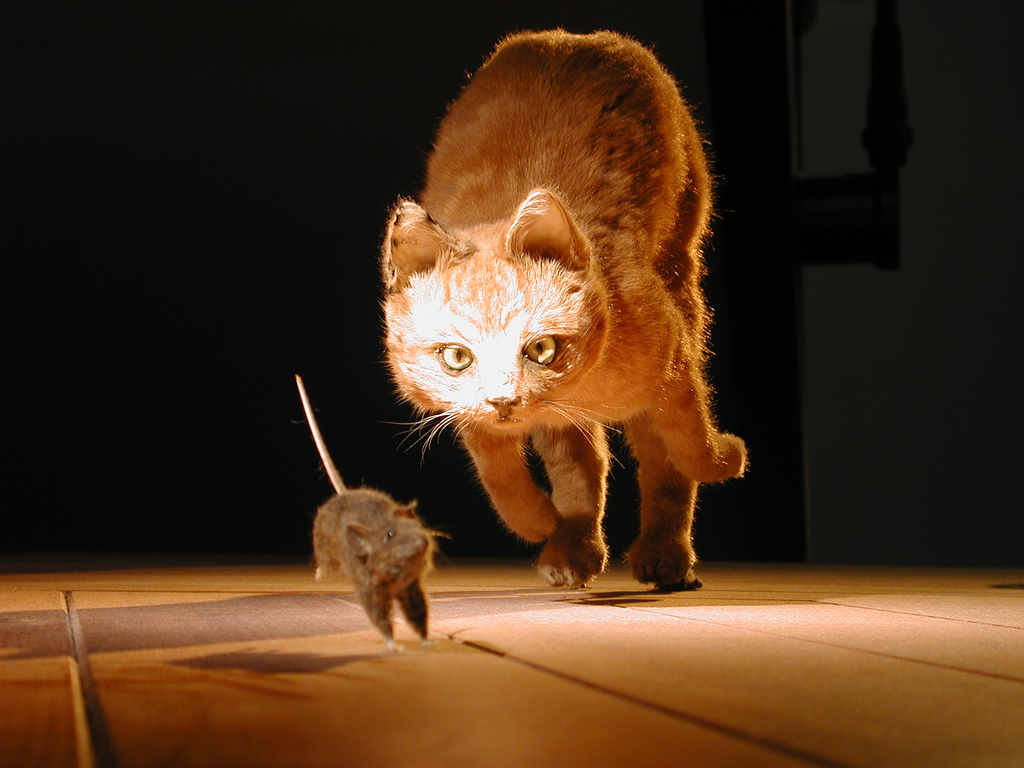
\includegraphics[scale=.1]{gfx/cat2.jpg}};
		\only<6->{\node[below = .5cm of screen, rectangle, draw, fill=gray!20!white] (message) {Message};}
		\only<6->{\draw[->, thick] (1.95,-2.5) -- (message);}
		\only<7->{\draw[->, dashed, thick, to path={|- (\tikztotarget)}] (message) edge (3.5,-4.5);}
		
	\end{tikzpicture}
	}
\end{backgroundblock}

\only<2>{
	\begin{backgroundblock}{33mm}{73mm}	
		\begin{tikzpicture}[level distance=25pt]
			\Tree [.NP ]
			
		\end{tikzpicture}
		
	\end{backgroundblock}
}

\only<3>{
	\begin{backgroundblock}{35mm}{73mm}	
		\begin{tikzpicture}[level 1/.style={level distance=5pt},
			level 2/.style={level distance=25pt}]
			\Tree [ [.NP ] [.VP V ] ]
			
		\end{tikzpicture}
		
	\end{backgroundblock}
}

\only<4>{
	\begin{backgroundblock}{35mm}{73mm}	
		\begin{tikzpicture}[level 1/.style={level distance=5pt},
			level 2/.style={level distance=25pt}]
			\Tree [ [.NP ] [.VP V NP ] ] ]
			
		\end{tikzpicture}
		
	\end{backgroundblock}
}

	\begin{backgroundblock}{40mm}{55mm}	
		\only<7>{
		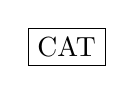
\begin{tikzpicture}[level 1/.style={level distance=15pt},
			level 2/.style={level distance=25pt}]
			\Tree [ [.NP  \edge[color=white]; \node[draw]{CAT}; ] [.VP \edge[dashed, color = gray!60!white]; {\color{gray!50!white}V} \edge[dashed, color = gray!60!white]; {\color{gray!50!white}NP} ] ] ]
			
		\end{tikzpicture}
	}	
	\only<8>{
	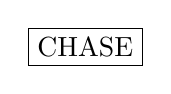
\begin{tikzpicture}[level 1/.style={level distance=15pt, sibling distance=1pt},
		level 2/.style={level distance=25pt}]
		\Tree [ \edge[dashed, color = gray!60!white];
				[.{\color{gray!50!white}NP} ]
					[.VP [.V \edge[color=white]; \node[draw]{CHASE}; ] {\color{gray!50!white}NP} 
					] 
				] 
		
	\end{tikzpicture}
	}	
	\only<9>{
	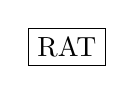
\begin{tikzpicture}[level 1/.style={level distance=20pt, sibling distance=20pt},
		level 2/.style={level distance=25pt}]
		\Tree [ \edge[dashed, color = gray!60!white];
				[.{\color{gray!50!white}NP} ] \edge[dashed, color = gray!60!white];
					[.{\color{gray!50!white}VP} \edge[dashed, color = gray!60!white]; {\color{gray!50!white}V} 
					 [.NP \edge[color=white]; \node[draw]{RAT}; ]
				] 
			] 
		
	\end{tikzpicture}
	}	
	\end{backgroundblock}




\end{frame}



\begin{frame}%{Image-description task}
	
	\only<1>{
		\begin{flushleft}
			\vspace{4cm}
			\Huge{\textbf{+}}
		\end{flushleft}
	}	
	
	\only<2>{
		\begin{backgroundblock}{20mm}{37mm}		
			
\includegraphics[scale=.35]{gfx/peter2}
		\end{backgroundblock}
		
		\begin{backgroundblock}{55mm}{36mm}		
			
\includegraphics[scale=.4]{gfx/073} 
		\end{backgroundblock}
		
		\begin{backgroundblock}{90mm}{37mm}		
			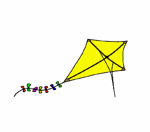
\includegraphics[scale=.4]{gfx/129}
		\end{backgroundblock}
	}
	
	\only<3>{
		\begin{backgroundblock}{20mm}{23mm}		
			
\includegraphics[scale=.35]{gfx/peter2}
		\end{backgroundblock}
		
		\begin{backgroundblock}{55mm}{22mm}		
			
\includegraphics[scale=.4]{gfx/073} 
		\end{backgroundblock}
		
		\begin{backgroundblock}{90mm}{52mm}		
			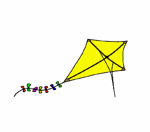
\includegraphics[scale=.4]{gfx/129}
		\end{backgroundblock}
	}
	
	
	\only<4>{
		\begin{center}
			{\huge\textit{The boy and the dog moved above the kite.}}
		\end{center}
	}
	
	
	
\end{frame}


%\blfootnote{\parencite{ martin2014working,martin2010planning, roeser2019advance, smi99, wag10,hardy2019age,hardy2020healthy,ferreira1991effects,levelt1981lexical,wheeldon2013,smith2001,konopka2012planning}}
\begin{frame}
	
	\newcommand{\ImageWidth}{11cm}
	\begin{tikzpicture}
		% draw horizontal line   
		\draw[thick, -Triangle] (0,-1) -- (\ImageWidth,-1) node[font=\scriptsize, below left=3pt and -8pt]{Time (in msecs)};
		
		\node[inner sep=0pt] (stim) at (1.5,-.1) 
		{\fcolorbox{black}{white}{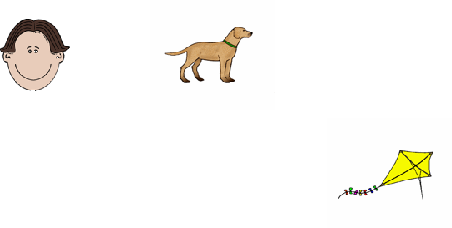
\includegraphics[scale=.351]{gfx/method/build/screen-3}}};
		
		\node[inner sep=0pt, visible on=<2->, right = 3cm of stim] (voice) 
		{
\includegraphics[scale=.2]{speech.jpeg}};
		
		% draw vertical lines
		\foreach \x in {0,1,...,8}
		    	\draw (\x cm,-1) -- (\x cm,-1.2);
    	
		\foreach \x/\descr in {0/0,1/200,2/400,3/600,4/700,5/800,6/900,7/1000,8/1200}
				\node[font=\scriptsize, text height=1.75ex, text depth=.5ex] at (\x,-1.4) {$\descr$};
		

		\draw[-Triangle,dashed,red!60!black,line width=2pt,visible on=<3->] (0,-2) -- +(8,0);
		
		% braces
		\draw [thick,decorate, color = white, visible on=<3->] (5,-2.15) -- +(-1,0)
		node [black,midway,below=4pt] {Onset latency};
		
		\draw[thick, dashed, visible on=<2->](0,-3) -- (0,.7) 
		node[font=\scriptsize] at (1.2,-3) {Stimulus onset};
		
		\draw[thick, dashed, visible on=<2->](8,-3) -- (8,.7) 
		node[font=\scriptsize] at (7,-3) {Voice onset};
		
	\end{tikzpicture}
	
\end{frame}

\begin{frame}
	
	\newcommand{\ImageWidth}{11cm}
	\begin{tikzpicture}

% draw horizontal line   
\draw[thick, -Triangle] (0,-1) -- (\ImageWidth,-1) node[font=\scriptsize, below left=3pt and -8pt]{Time (in msecs)};

\node[inner sep=0pt] (stim) at (1.5,-.1) 
{\fcolorbox{black}{white}{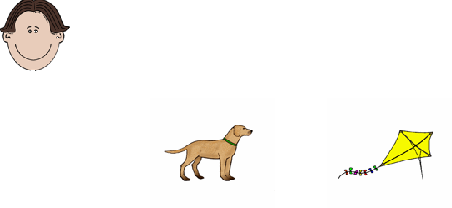
\includegraphics[scale=.351]{gfx/method/build/screen-4}}};

\node[inner sep=0pt, right = 2cm of stim] (voice) 
{
\includegraphics[scale=.2]{speech.jpeg}};

% draw vertical lines
\foreach \x in {0,1,...,8}
\draw (\x cm,-1) -- (\x cm,-1.2);

\foreach \x/\descr in {0/0,1/200,2/400,3/600,4/700,5/800,6/900,7/1000,8/1200}
\node[font=\scriptsize, text height=1.75ex, text depth=.5ex] at (\x,-1.4) {$\descr$};

\draw[-Triangle,dashed,red!60!black,line width=2pt] (0,-2) -- +(7,0);

% braces
\draw [thick,decorate, color = white] (4,-2.15) -- +(-1,0)
node [black,midway,below=4pt] {Onset latency};

\draw[thick, dashed](0,-3) -- (0,.7) 
node[font=\scriptsize] at (1.2,-3) {Stimulus onset};

\draw[thick, dashed](7,-3) -- (7,.7) 
node[font=\scriptsize] at (6,-3) {Voice onset};

		
	\end{tikzpicture}
	
\end{frame}


%\begin{frame}{Planning scope in sentence production\blfootnote{\shortciteA<e.g.>{ martin2014working, roeser2018advance, smi99}} }

\begin{frame}{Preplanning scope involves syntax}

\begin{itemize}
	\item[1.] \textbf{The boy and the dog} moved above the kite.
	\item[2.] \textbf{The boy} moved above the dog and the kite.
\end{itemize}
\vfill
\begin{itemize}
		\item Frequently reproduced effect \parencite[e.g.][]{martin2014working,smi99,wag10}.
		\item ``Phrase as default planning scope'' \parencite{martin2010planning}
		\item NP syntax is planned before production onset.
		\item Lexical scope is smaller \parencite{gri01} and flexible \parencite{wheeldon2013}.
\end{itemize}

\end{frame}


\begin{comment}
\begin{frame}{Advance planning involves syntax}
\begin{itemize}
	\item Subordination vs coordination with conflicting results \parencite{not07, all07}.
	\begin{itemize}
		\item[2a.] The A with the B is \dots
		\item[2b.] The A and the B are \dots
	\end{itemize}		
	\item Syntactic proximity \parencite{lee13}.
	\begin{itemize}
		\item[3a.] Click on [[the fork of the king] below the apple]
		\item[3b.] Click on [the fork of [the king below the apple]]
	\end{itemize}
	\item Lexical scope is flexible \parencite{wheeldon2013}.
\end{itemize}
\end{frame}
\end{comment}


\begin{frame}{Implication of the standard statistical treatment}

	\begin{itemize}
		\item \uncover<1->{Statistical models used (LMM, ANOVA) map onto a deterministic syntax-driven model.}
		\item \uncover<2->{Systematic difference between simple and conjoined NPs.} 	
		\item \uncover<3->{Under these statistical models, the following alternative hypothesis couldn't be tested.}
	\end{itemize}

\end{frame}

% Under what circumstances would it be optional to plan phrase syntax or not
% Alternative: syntax planning is non-deterministic
% a. a syntactic route is available as well as a lexical route
% b. a lexical-guided production system can in in principle prepare larger chunks before utterance onset for non-syntactic reasons (distance between nouns; visual grouping).


\begin{frame}{Alternative hypothesis}

\begin{itemize}
	\item \textbf{Preplanning beyond the first noun is more likely but not obligated by the phrase syntax} because, for example, \dots 
	\item[1.] Fluency pressure requires preplanning of B in \textit{The A and the B moved \dots} if there is not enough time to plan B in parallel to articulation \parencite{all07,griffin2003reversed}.
	\item[2.] Activation of phrase syntax or use of the syntactic route is non-deterministic.
\end{itemize}

\end{frame}



	
\begin{frame}{Research focus}

\begin{itemize}
	\item Direct comparison of two hypothesis.
	\item[i.] \uncover<1->{Phrase scope obligated by the production system, leading to a systematic slowdown for conjoined NPs.}
	\item[ii.] \uncover<1->{Preplanning beyond the first noun is more likely in conjoined NPs but not obligated by the production system.} 


\end{itemize}

\end{frame}


\begin{frame}{Pooled re-analysis}


\begin{itemize}
	\item Stimulus-to-onset latencies
	\item[a.] \textbf{Conjoined NPs:} \textit{The boy and the dog moved above the kite.}
	\item[b.] \textbf{Simple NPs:} \textit{The boy moved above the dog and the kite.}	
\end{itemize}


\begin{itemize}
	\item \textcite{hardy2019age}: 90 ppts; 36 items
	\item \textcite{hardy2020healthy}: 105 ppts; 80 items
	\item \textcite{martin2010planning}: 3$\times$12 ppts; 2$\times$48 and 1$\times$64 items
	\item \textcite{roeser2019advance}: 3$\times$32 ppts; 96 items 
\end{itemize}


\end{frame}


\begin{frame}{Data overview}
	\begin{flushright}
		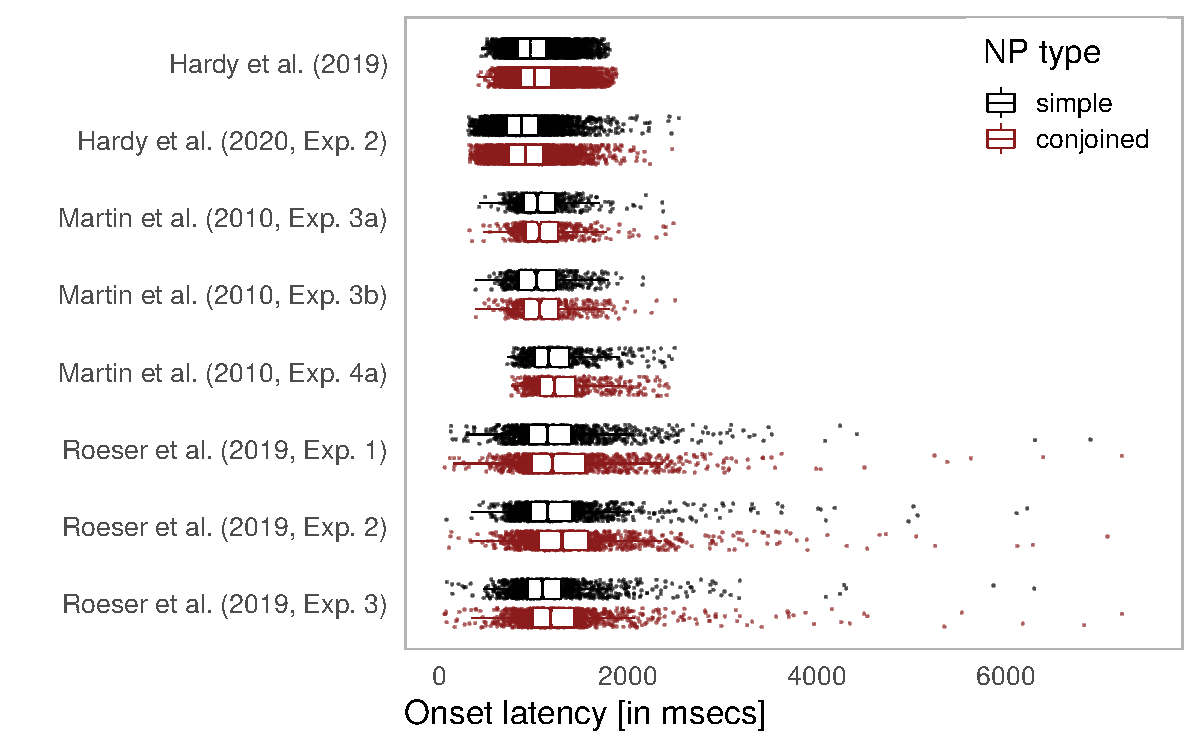
\includegraphics[scale=.5]{metaraw.pdf}
	\end{flushright}
\end{frame}






\begin{frame}[fragile]{Model overview}

\begin{minipage}[t]{.53\textwidth}
\uncover<-2>{
\begin{enumerate}
		\item Null LMM
		\item \textbf{LMM (NP effect)}
		\item LMM (unequal variance)
		\item Null mixture model
		\item \textbf{Mixture model}
\end{enumerate}
\vfill
\begin{itemize}
 	\item Stan code based on \textcite{sorensen2016bayesian} and \textcite{vasishth2017}; also \textcite{vasishth2017feature}.
\end{itemize}

}
\end{minipage}
\hfill
\begin{minipage}[t]{.45\textwidth}
\uncover<2->{
\begin{itemize}
	\item $LogNormal$ distribution with mean $\mu$ and error variance $\sigma_e^2$
	\item Random intercepts 
	\begin{itemize}
		\item participants: $u_i \sim Normal(0, \sigma_u^2)$
		\item items: $w_j \sim Normal(0, \sigma_w^2)$
	\end{itemize}
	\item Weakly informative priors \parencite{mcelreath2016statistical}
\end{itemize}
}
\end{minipage}
	
\end{frame}

\begin{frame}[fragile]{Null model (null hypothesis)}
	
		\begin{equation*}
			\begin{aligned}	
				y_{ij} \sim LogNormal(\mu_{ij}, \sigma_e^2) \\
				\mu_{ij} = \alpha + u_i + w_j\\
			\end{aligned}
		\end{equation*}
\end{frame}


\begin{frame}[fragile]{Meta null model (null hypothesis)}
	
		\begin{equation*}
			\begin{aligned}	
				y_{ijk} \sim LogNormal(\mu_{ijk}, \sigma_{e_k}^2) \\
				\mu_{ijk} = \alpha_k + u_i + w_j\\
				\alpha_k = \alpha_{\mu} + \alpha_{\tau} \cdot \alpha_{\eta_k}\\
			\end{aligned}
		\end{equation*}
		\begin{small}	
			\begin{itemize}
				\item For $k = 1, \dots, K$ where $K$ is the number of studies.
				\item $\alpha_k$ is the latency coefficient for the $k$th study.
				\item $\alpha_{\mu}$ is the pooled latency coefficient.
				\item Non-centred parametrisation for $\alpha_k$ \parencite{gelman2014}.
			\end{itemize}
		\end{small}
\end{frame}


\begin{frame}[fragile]{Meta LMM (standard analysis)}
			
	\begin{equation*}
		\begin{aligned}	
			y_{ijk} \sim LogNormal(\mu_{ijk}, \sigma_{e_k}^2)\\
			\mu_{ijk} = \alpha_k + \beta_k \cdot x_{[0,1]} + u_i + w_j\\
			\alpha_k = \alpha_{\mu} + \alpha_{\tau} \cdot \alpha_{\eta_k}\\
			\beta_k = \beta_{\mu} + \beta_{\tau} \cdot \beta_{\eta_k}\\
		\end{aligned}	
	\end{equation*}		
	\begin{small}	
		\begin{itemize}
			\item $x=0$ for simple NPs; $x=1$ for conjoined NPs.
			\item $\beta_k$ is the latency change for conjoined NPs for the $k$th study.
			\item $\beta_{\mu}$ is the pooled latency change for conjoined NPs.
		\end{itemize}
	\end{small}
	
\end{frame}


\begin{frame}[fragile]{Mixture model (alternative hypothesis)}
	
	\begin{equation*}
		\begin{aligned}
		y_{ij} \sim \theta_{NP} \cdot LogNormal(\mu_{ij} + \delta, \sigma_{e'}^2) + \\
			(1 - \theta_{NP}) \cdot LogNormal(\mu_{ij}, \sigma_{e}^2) \\
			\mu_{ij} = \alpha + u_i + w_j\\
			\text{constraint: }\delta>0\\
			\sigma_{e'}^2 > \sigma_{e}^2 
		\end{aligned}
	\end{equation*}

\uncover<2>{
	\begin{small}
		\begin{itemize}
%			\item $\mu_{ij}$ defined as before.
			\item Probability of long latencies $\theta$ by NP type.
			\item $\mu$ and $\sigma^2$ constant across NP type.
		\end{itemize}
	\end{small}		
}
	
\end{frame}

\begin{frame}[fragile]{Meta mixture model (alternative hypothesis)}

	\begin{equation*}
		\begin{aligned}
		y_{ijk} \sim \theta_{{NP}_k} \cdot LogNormal(\mu_{ijk} + \delta_k, \sigma_{e'_k}^2) + \\
			(1 - \theta_{{NP}_k}) \cdot LogNormal(\mu_{ijk}, \sigma_{e_k}^2) \\
			\mu_{ijk} = \alpha_k + u_i + w_j\\
			\theta_{{NP}_k} = Logit^{-1}(\phi_{{NP}_k})\\
%			\theta_{{NP}} = Logit^{-1}(\phi_{_{\mu_{NP}}})\\		
			\phi_{{NP}_k} \sim Normal(\phi_{\mu_{NP}}, \phi_{\tau}^2)\\
			\delta_k \sim Normal(\delta_{\mu}, \delta_{\tau}^2)\\
			\text{constraint: }\delta_k>0\\
		\end{aligned}
	\end{equation*}
	
	\begin{small}	
		\begin{itemize}
			\item $\alpha_{k}$, $\sigma_{e'_k}^2$, $\sigma_{e_k}^2$ defined as before.
			\item Pooled coefficient for parameters: $\theta_{NP}$, $\delta$
%			\item Inverse-logit for continuous prior on mixing proportion.
		\end{itemize}
	\end{small}
	
\end{frame}


\begin{frame}[fragile]{Meta LMM (unequal variance)}
	\begin{equation*}
		\begin{aligned}
		y_{ijk} \sim
			\begin{dcases*} 
				LogNormal(\mu_{ijk}, \sigma_{e_k}^2), &  if NP$_{ijk}$ = simple\\
				LogNormal(\mu_{ijk} + \beta_k, \sigma_{e'_k}^2) & else if NP$_{ijk}$ = conjoined\\
			\end{dcases*}\\
		\mu_{ijk} = \alpha_k + u_i + w_j\\
		\alpha_k = \alpha_{\mu} + \alpha_{\tau} \cdot \alpha_{\eta_k}\\
		\beta_k = \beta_{\mu} + \beta_{\tau} \cdot \beta_{\eta_k}\\
		\text{constraint: }\sigma_{e_k}^2>0\\
		\sigma_{e'_k}^2 > \sigma_{e_k}^2
		\end{aligned}
	\end{equation*}
	
	
\end{frame}


\begin{comment}
\begin{frame}{Predictions}

\begin{itemize}
	\uncover<-1>	{\item Standard analysis (LMM): Conjoined NPs cause a systematic slowdown in onset latencies, implying that phrase syntax is obligated by the production system.}
	\uncover<2>	{\item Alternative analysis (MoG): Conjoined NPs show a larger probability for longer onset latencies which, however, remain the minority; hence, preplanning syntax is not obligated by the production system.}
\end{itemize}

\end{frame}
\end{comment}




	
\begin{frame}{NP effect (LMM)}
	\begin{flushright}
		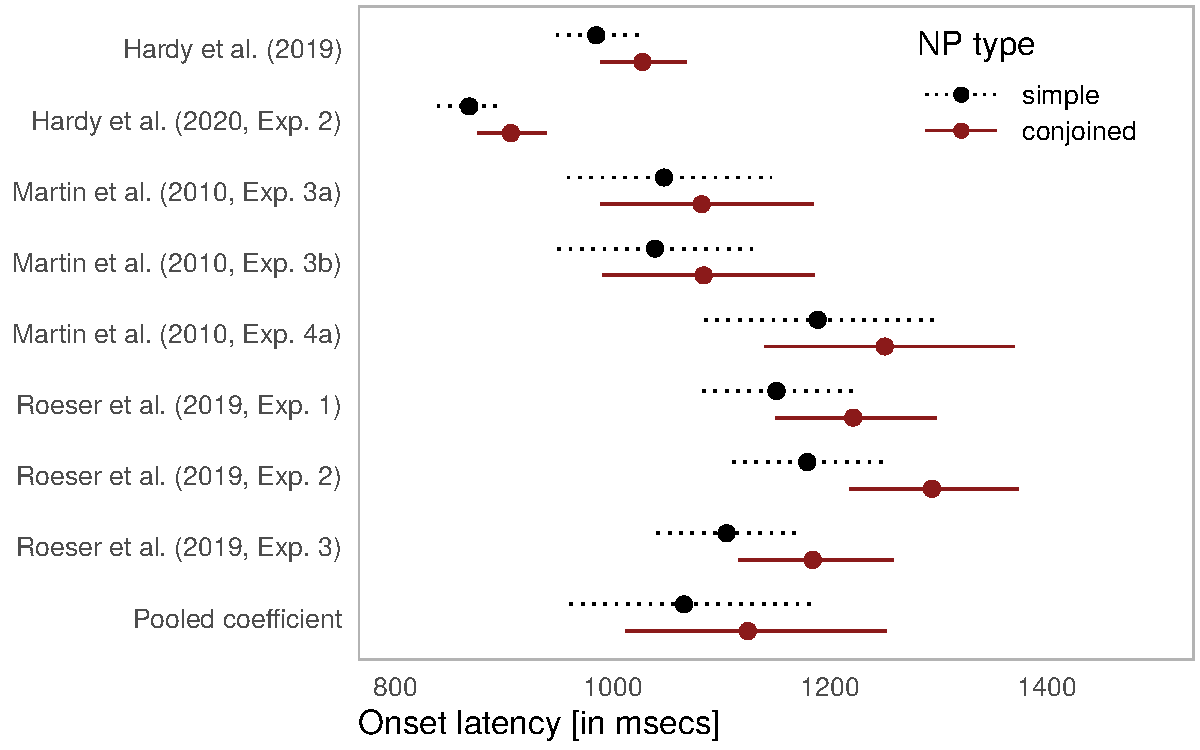
\includegraphics[scale=.5]{NPmeta.pdf}
	\end{flushright}
\end{frame}


\begin{frame}{NP effect (LMM)}
	\begin{flushright}	
		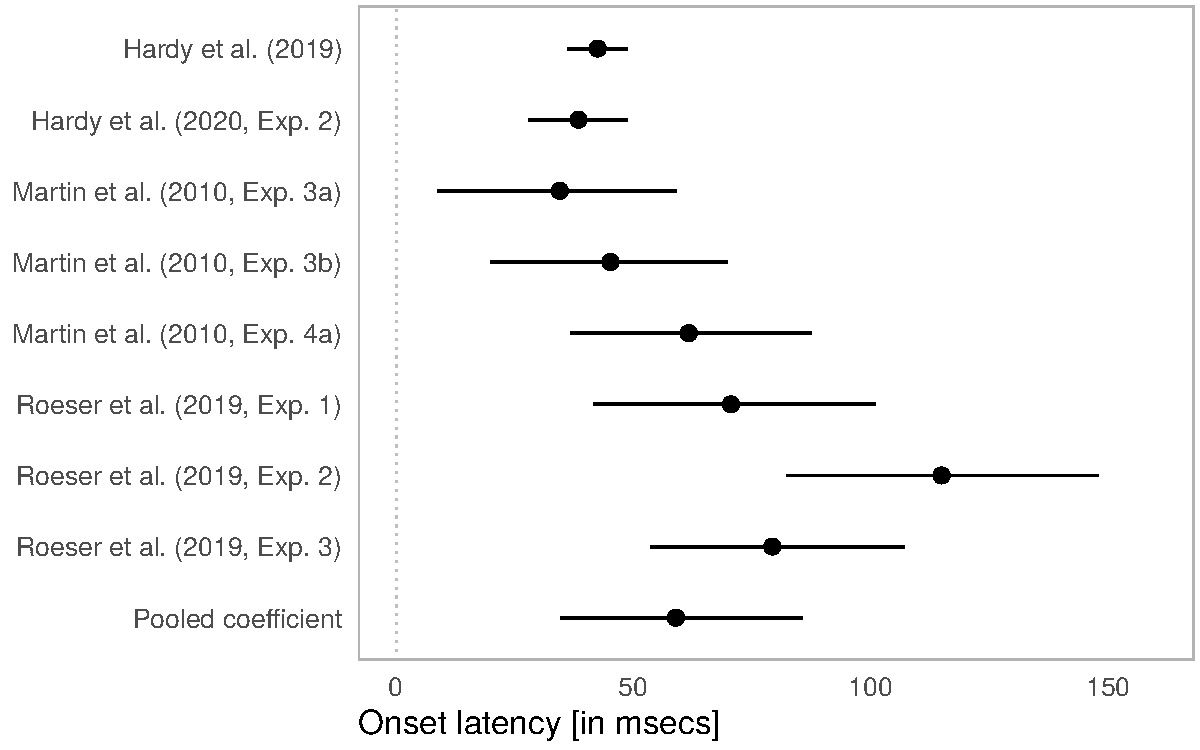
\includegraphics[scale=.5]{NPmetadiff.pdf}
	\end{flushright}
\end{frame}



\begin{frame}{Model comparisons}
\begin{scriptsize}
% latex table generated in R 4.0.2 by xtable 1.8-4 package
% Tue Aug 18 15:17:51 2020
	\begin{table}[ht]
	\centering
	\caption{\scriptsize{Predictive performance estimated as the \textit{expected log pointwise predictive density} ($\widehat{elpd}$) \parencite{vehtari2015pareto, vehtari2017practical}. Models are ordered by predictive performance (model with highest predictive performance in top row)}. Standard error in parentheses.}
		\begin{tabular}{lrrl}
		\toprule
		Models & $\updel\widehat{elpd}$ & $\widehat{elpd}$ & Description \\ [1ex]
		\midrule
		\rowcolor{yellow!40!white}MoG-1 & -- & -201,486 (176) & Mixing proportions by NP \\ [1ex]
  		MoG-0 & -15 (8) & -201,500 (176)  & Null model \\ [1ex]
 		\rowcolor{yellow!40!white}LMM-1 & -1,006 (97) & -202,492 (214) & NP effect \\ [1ex]
  		LMM-0 & -1,192 (92) & -202,678 (212) & Null model \\ [1ex]
 		LMM-2 & -3,537 (214) & -205,022 (307) & Unequal variance \\ [1ex]
		\bottomrule
		\end{tabular}\\
		\textit{Note.} LMM = Linear mixed effects model; MoG = Mixture of Gaussians 
	\end{table}
\end{scriptsize}
\end{frame}



\begin{frame}{Probability of long latencies (MoG)}

	\begin{flushright}
		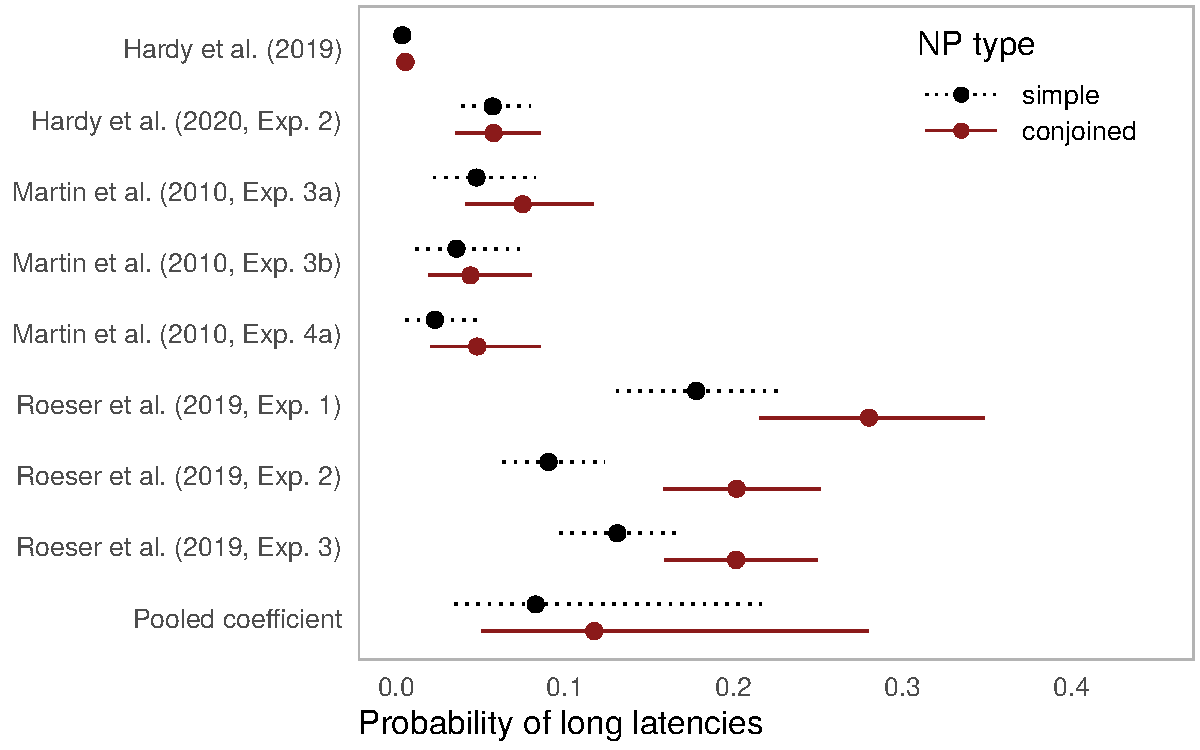
\includegraphics[scale=.5]{mogmeta.pdf}
	\end{flushright}


\end{frame}
	\begin{frame}{Bridge to follow-up experiments}

\setlength{\leftmargini}{0.5cm}
\setlength{\leftmarginii}{0.5cm}
\begin{itemize}
	\item Slowdown for conjoined NPs is better explained by a larger, yet relatively small, probability of long latencies.
	\item Most studies in our pool included other manipulations.
%	\item Different pattern for \textcite{hardy2019age,hardy2020healthy} compared to  \textcite{martin2010planning} and \textcite{roeser2019advance}.%; possibly because of data trimming thresholds.
\end{itemize}
\begin{itemize}
	\item[$\bullet$] \textbf{Experiment 1:} 
	\begin{itemize}
		\item Reproduce analysis after \dots
		\item[i.] Reducing the manipulation to simple and conjoined NPs.
		\item[ii.] Controlling image names
	\end{itemize}
	\item[$\bullet$] \textbf{Experiment 2:} 
	\begin{itemize}
		\item Assess impact of visual manipulation \parencite[as in][]{martin2010planning}.
	\end{itemize}
\end{itemize}

\end{frame}
	\begin{frame}{Methods}

\begin{backgroundblock}{30mm}{5mm}
	\begin{tikzpicture}[framed,background rectangle/.style={thick, rounded corners, draw=black}]
		\node[inner sep=1pt] (screen) at (10,-5)
    		{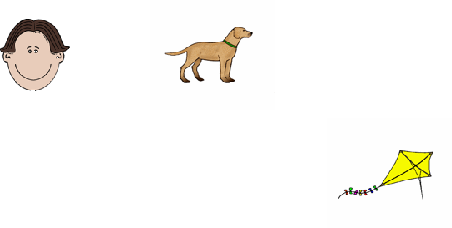
\includegraphics[scale=.5]{gfx/method/build/screen-3}};   		
    		\node[font = \tiny, below = 0cm of screen] {Condition 1: A and B moved above C};
	\end{tikzpicture}
\end{backgroundblock}

\begin{backgroundblock}{75mm}{5mm}
	\begin{tikzpicture}[framed,background rectangle/.style={thick, rounded corners, draw=black}]
		\node[inner sep=3.5pt] (screen) at (10,-5)
    		{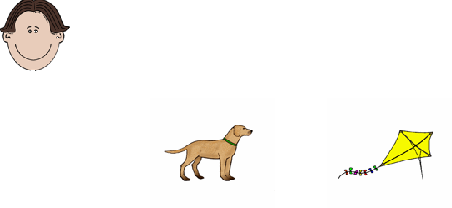
\includegraphics[scale=.5]{gfx/method/build/screen-4}};   			    					\node[font = \tiny, below = 0cm of screen] {Condition 2: A moved above B and C};
	\end{tikzpicture}
\end{backgroundblock}

\vspace{2cm}
\begin{footnotesize}
\begin{minipage}[t]{.55\textwidth}
\setlength{\leftmargini}{0.5cm}
\setlength{\leftmarginii}{0.5cm}
\begin{itemize}
	\item \textbf{Experiment 1:}
	\begin{itemize}
		\item[1a.] \uncover<2->{\textbf{Peter and the dog} moved above the kite}
		\item[1b.] \uncover<2->{\textbf{Peter} moved above the dog and the kite}
		\item \uncover<2->{78 ppts (after cleaning)}
	\end{itemize}
	\item \textbf{Experiment 2:}
	\begin{itemize}
		\item[2.] \uncover<3->{Peter, the dog, the kite}
		\item \uncover<3->{45 ppts (after cleaning)}
	\end{itemize}
\end{itemize}
\end{minipage}
\hfill
\begin{minipage}[t]{.4\textwidth}
\begin{itemize}
	\item \uncover<4>{First noun: \textit{Peter} or \textit{Tania}}
	\item \uncover<4>{Movement: up or down}
	\item \uncover<4>{48 items; 96 fillers; 6 practice trials}
	\item \uncover<4>{Image names: high frequency and naming agreement.}
\end{itemize}
\end{minipage}
\end{footnotesize}

\end{frame}
	\begin{frame}{Onset latencies}
	\begin{center}	
		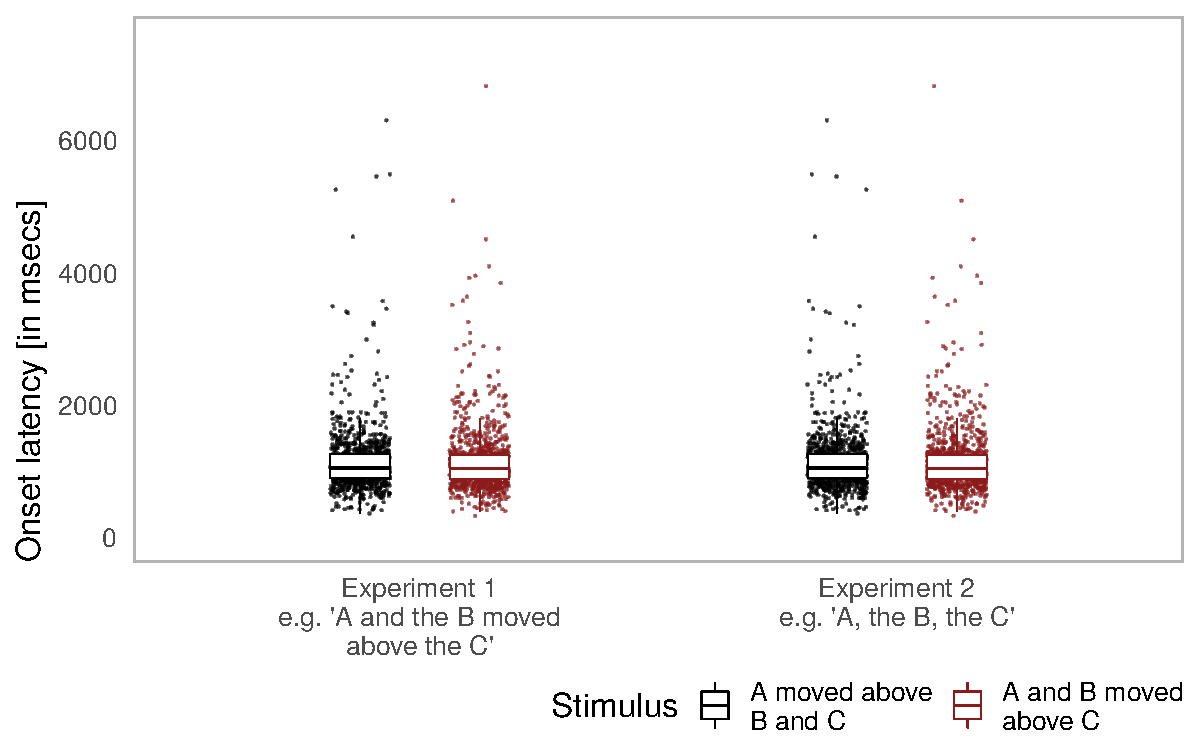
\includegraphics[scale=.5]{expsraw.pdf}
	\end{center}
\end{frame}

\begin{frame}{NP-type effect (LMM)}

\begin{tikzpicture}
    \draw (0, 0) node[inner sep=0,anchor=west] {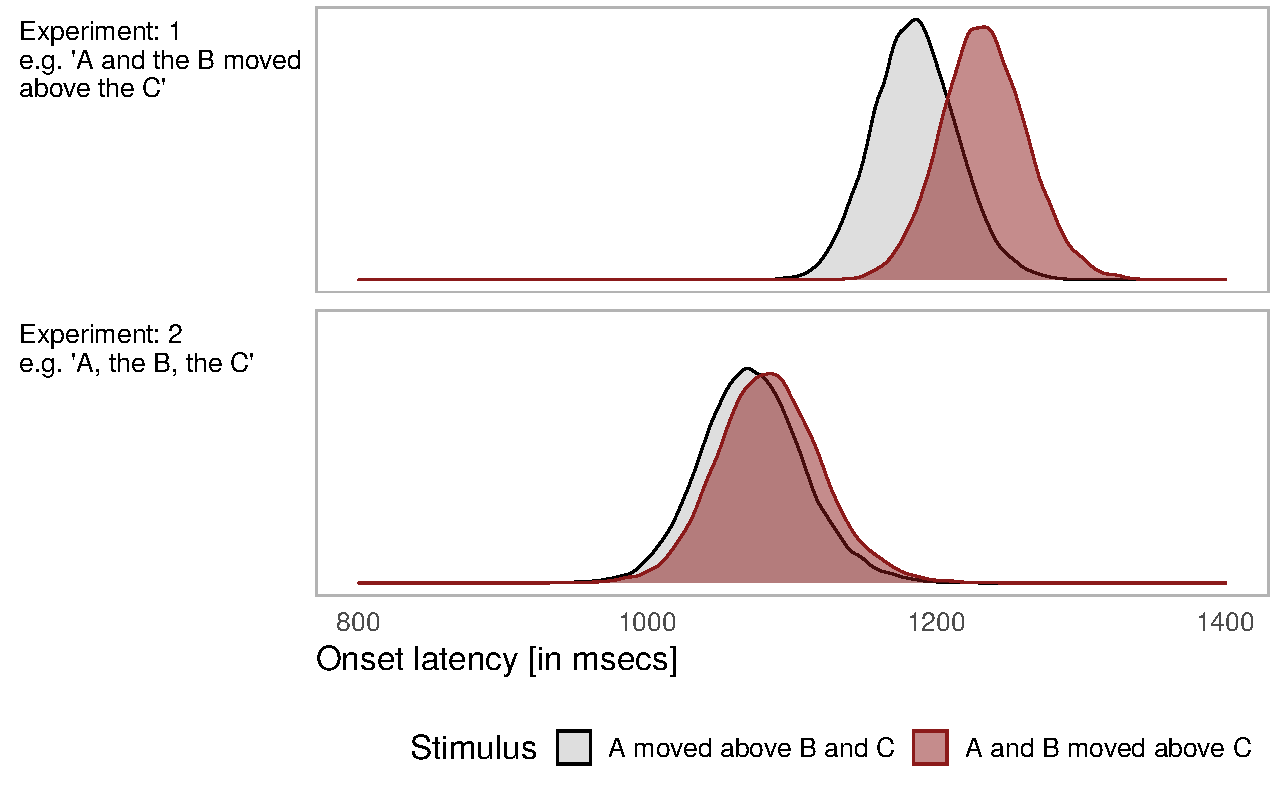
\includegraphics[scale=.5]{NPexp.pdf}};
    \draw (2.75, 2.9) node[font=\tiny,anchor=west] {LMM-1 -- LMM-0: $\updel\widehat{elpd}=$-6 (4)};
    \draw (2.75, 2.5) node[font=\tiny,anchor=west] {LMM-1: $\widehat{elpd}=$-22,364 (107)};
    \draw (10.75, .35) node[font=\tiny,anchor=east] {LMM-1 -- LMM-0: $\updel\widehat{elpd}=$1 (1)};
    \draw (10.75, -.05) node[font=\tiny,anchor=east] {LMM-1: $\widehat{elpd}=$-14,451 (80)};
\end{tikzpicture}

\end{frame}

\begin{frame}{Probability of long latencies (MoG)} 

\begin{tikzpicture}
    \draw (0, 0) node[inner sep=0,anchor=west] {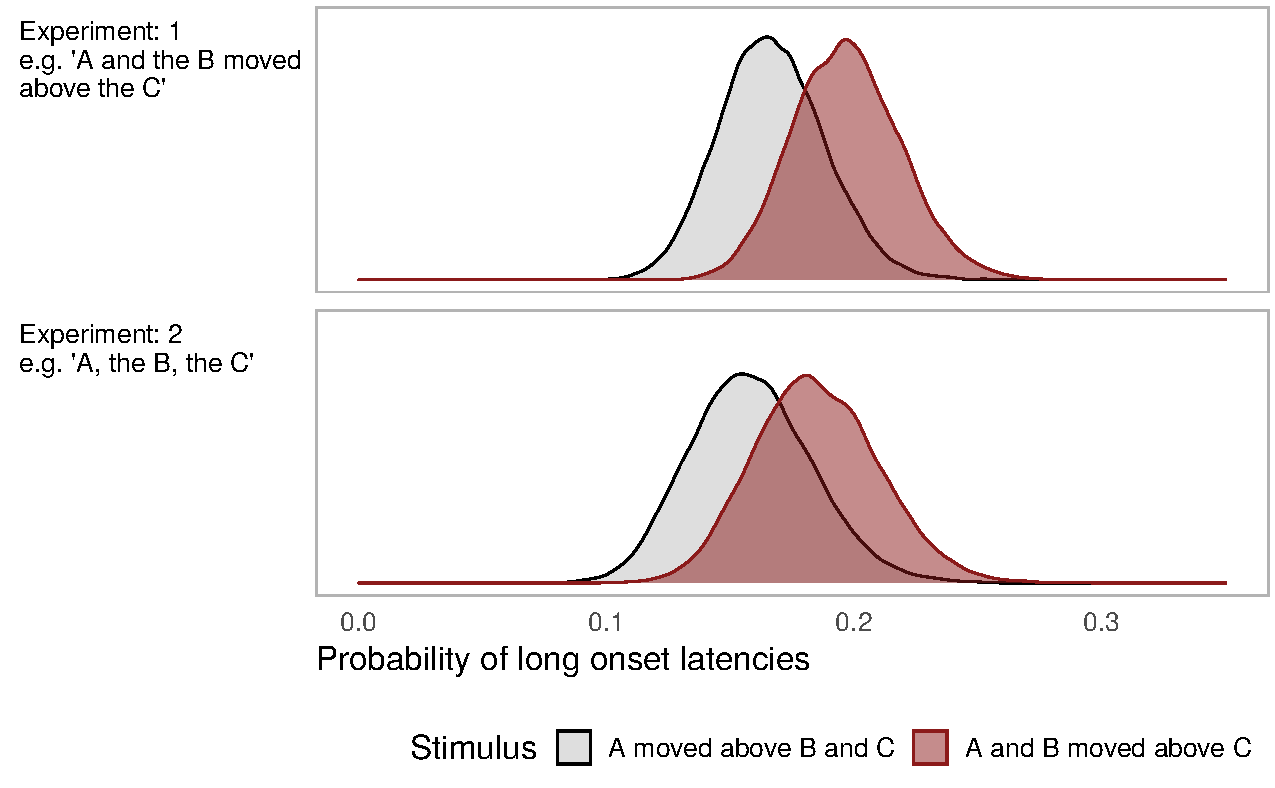
\includegraphics[scale=.5]{NPexpmog.pdf}};
    \draw (10.75, 2.95) node[font=\tiny,anchor=east] {MoG-1 -- LMM-1: $\updel\widehat{elpd}=$-513 (56)};
    \draw (10.75, 2.55) node[font=\tiny,anchor=east] {MoG-1: $\widehat{elpd}=$-21,851 (74)};
    \draw (10.75, .45) node[font=\tiny,anchor=east] {MoG-1 -- LMM-1: $\updel\widehat{elpd}$=-362 (44)};
    \draw (10.75, .05) node[font=\tiny,anchor=east] {MoG-1: $\widehat{elpd}$=-14,089 (57)};
\end{tikzpicture}

\end{frame}

	% summary of claim

\begin{frame}{Summary}
	\begin{itemize}
		\item Evidence against the phrase-as-planning-unit hypothesis: preplanning NP syntax is not obligated by the language production system.
		\item Instead, the slowdown for conjoined NPs \parencite[as in][]{martin2010planning,smi99} is better explained by a larger tendency to exhibit long onset latencies.
	\end{itemize}
\end{frame}

\begin{frame}{Alternative explanations}
	\begin{itemize}
		\item Preplanning scope is in-line with non-deterministic theories of language production.		
		\item Together with Exp.~2, results suggest that the slowdown observed in a subset of trials origins during visual rather than grammatical encoding. 
		\item Both a relational and non-relational route are available during high level encoding \parencite{kuchinsky2011reversing,konopka2014priming}. 
%		\item[i.] Lexical: avoidance of intra-sentential pausing.
%		\item[ii.] Syntactic: correction of incorrectly activated NP syntax.
%		\item[iii.] Both: use of syntactic route, instead of a lexical route, leads to a slowdown in conjoined NPs but not in simple NPs. 
	\end{itemize}
\end{frame}


	\begin{frame}
	
	\begin{center}
		{\huge Thank you for listening!}\\ $\phantom{foo}$ \\
	\end{center}
	
	\dots and \textbf{Randi Martin}, \textbf{Jason Crowther}, and \textbf{Sophie Hardy} (et al.) for sharing their data,
	
	\dots and \textbf{Dora Kramar} and \textbf{Andra Tanasescu} for supporting the data collection.

	\begin{center}
		email: \url{jens.roeser@ntu.ac.uk}\\ 
		\url{nottinghamtrent.academia.edu/JensRoeser}\\
		\textit{R} and \textit{Stan} code: \url{github.com/jensroes/NP-effect}\\
	\end{center}		
		
	\begin{tikzpicture}[node distance=1cm,remember picture,overlay]
		
	% nodes
	\node[anchor = north] (B) at (6, 1) {$ $};
	\node[below left = .1cm and 4.25cm of B] (A) {
\includegraphics[scale=.35]{gfx/github}};

	% arrows
	\draw[->, ultra thick, red!60!black, to path={|- (\tikztotarget)}]
	(B) to [out=260,in=335](A);
		
	\end{tikzpicture}
	
		
\end{frame}

	%-------------------------------------------------------------------------
% REFERENCES
%-------------------------------------------------------------------------
\renewcommand*{\bibfont}{\scriptsize}
\setbeamertemplate{bibliography item}{}
\begin{frame}[allowframebreaks]{References}
	
%	\bibliographystyle{apa}
%	\bibliographystyle{apacite}
%	\bibliography{refeferences}
\printbibliography
	
	
\end{frame}
	
	\begin{frame}[fragile]{Meta LMM}
			
	\begin{equation*}
		\begin{aligned}	
			y_{ijk} \sim LogNormal(\mu_{ijk}, \sigma_{e_k}^2)\\
			\mu_{ijk} = \alpha_k + \beta_k \cdot x_{[0,1]} + u_i + w_j\\
			\alpha_k = \alpha_{\mu} + \alpha_{\tau} \cdot \alpha_{\eta_k}\\
			\beta_k = \beta_{\mu} + \beta_{\tau} \cdot \beta_{\eta_k}\\
			\text{constraint: }\sigma_{e_k}^2>0\\
		\end{aligned}	
	\end{equation*}		
	\begin{small}	
		\begin{itemize}
			\item $x=0$ for simple NPs; $x=1$ for conjoined NPs.
		\end{itemize}
	\end{small}
	
\end{frame}

\begin{frame}[fragile]{Meta LMM (unequal variance)}
	\begin{equation*}
		\begin{aligned}
			y_{ijk} \sim
			\begin{dcases*} 
				LogNormal(\mu_{ijk}, \sigma_{e_k}^2), &  if NP$_{ijk}$ = simple\\
				LogNormal(\mu_{ijk} + \beta_k, \sigma_{e'_k}^2) & else if NP$_{ijk}$ = conjoined\\
			\end{dcases*}\\
			\mu_{ijk} = \alpha_k + u_i + w_j\\
			\alpha_k = \alpha_{\mu} + \alpha_{\tau} \cdot \alpha_{\eta_k}\\
			\beta_k = \beta_{\mu} + \beta_{\tau} \cdot \beta_{\eta_k}\\
			\text{constraint: }\sigma_{e_k}^2>0\\
			\sigma_{e'_k}^2 > \sigma_{e_k}^2
		\end{aligned}
	\end{equation*}

\end{frame}


\begin{frame}[fragile]{Meta mixture model (alternative hypothesis)}

	\begin{equation*}
		\begin{aligned}
		y_{ijk} \sim \theta_{{NP}_k} \cdot LogNormal(\mu_{ijk} + \delta_k, \sigma_{e'_k}^2) + \\
			(1 - \theta_{{NP}_k}) \cdot LogNormal(\mu_{ijk}, \sigma_{e_k}^2) \\
			\mu_{ijk} = \alpha_k + u_i + w_j\\
			\alpha_k = \alpha_{\mu} + \alpha_{\tau} \cdot \alpha_{\eta_k}\\
			\theta_{{NP}_k} = Logit^{-1}(\phi_{{NP}_k})\\
			\theta_{\mu_{NP}} = Logit^{-1}(\phi_{_{\mu_{NP}}})\\		
			\phi_{{NP}_k} \sim Normal(\phi_{\mu_{NP}}, \phi_{\tau}^2)\\
			\delta_k \sim Normal(\delta_{\mu}, \delta_{\tau}^2)\\
			\text{constraint: }\delta_k, \sigma_{e_k}^2, \phi_{\tau}, \delta_{\tau}>0\\
			\sigma_{e'_k}^2 > \sigma_{e_k}^2 
		\end{aligned}
	\end{equation*}
	
\end{frame}



	
\begin{frame}{Data overview (pooled data)}
	\begin{flushright}
		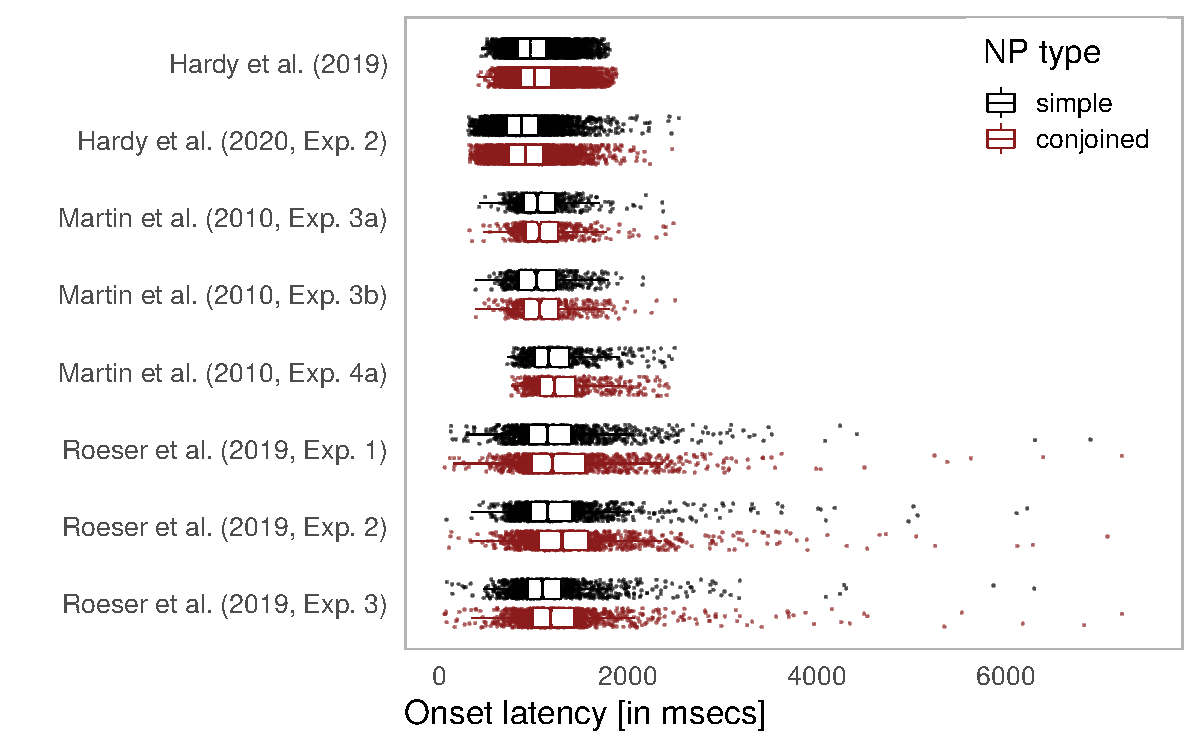
\includegraphics[scale=.5]{metaraw.pdf}
	\end{flushright}
\end{frame}


	\begin{frame}{Data overview (Experiments 1\& 2)}
	\begin{center}	
		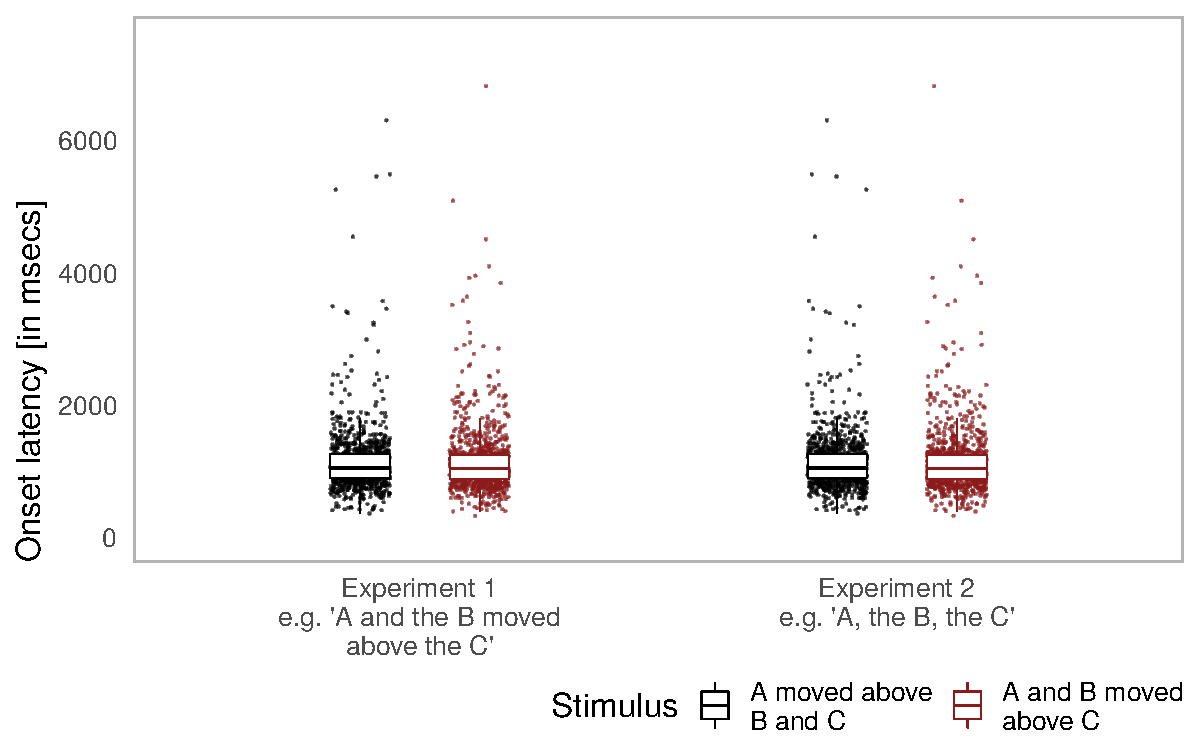
\includegraphics[scale=.5]{expsraw.pdf}
	\end{center}
\end{frame}
	\begin{frame}{Onset-latency coefficients (meta mixture components)} 
	\begin{center}	
		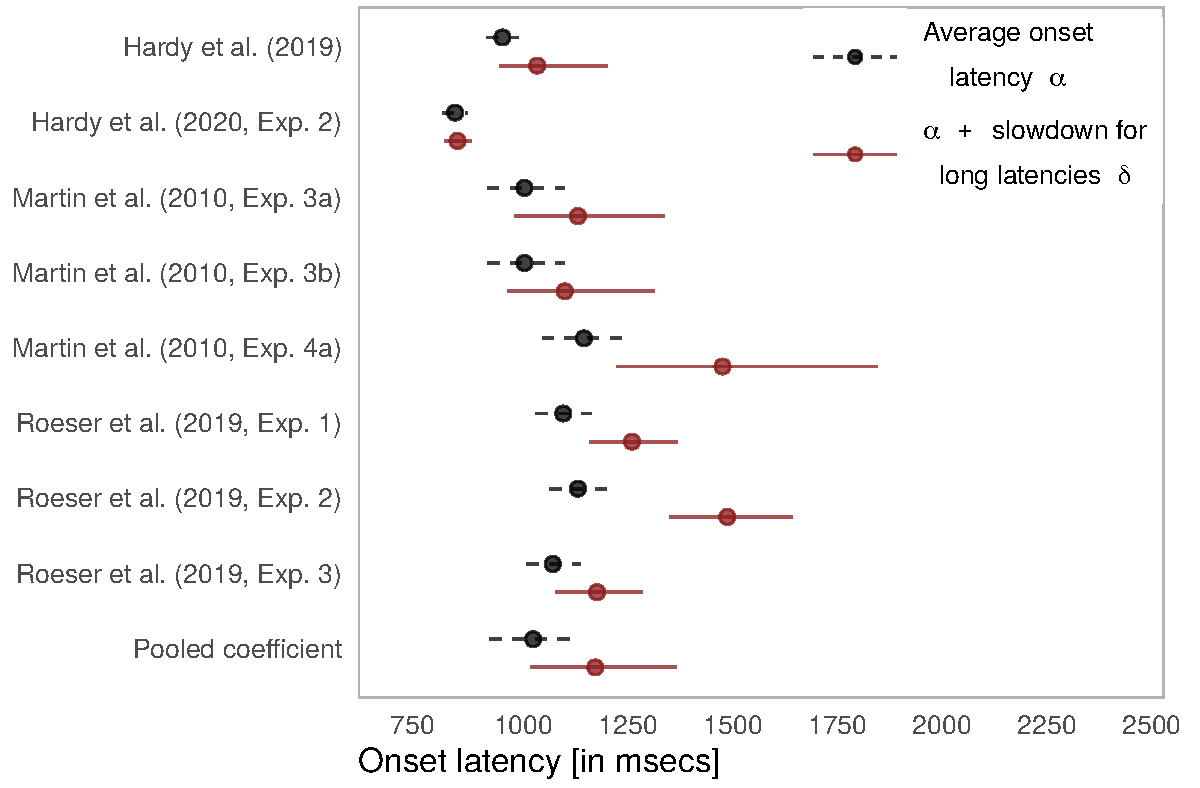
\includegraphics[scale=.5]{NPmetamoglong.pdf}
	\end{center}
\end{frame}

	\begin{frame}{Onset-latency coefficients (mixture components)} 
	\begin{center}	
		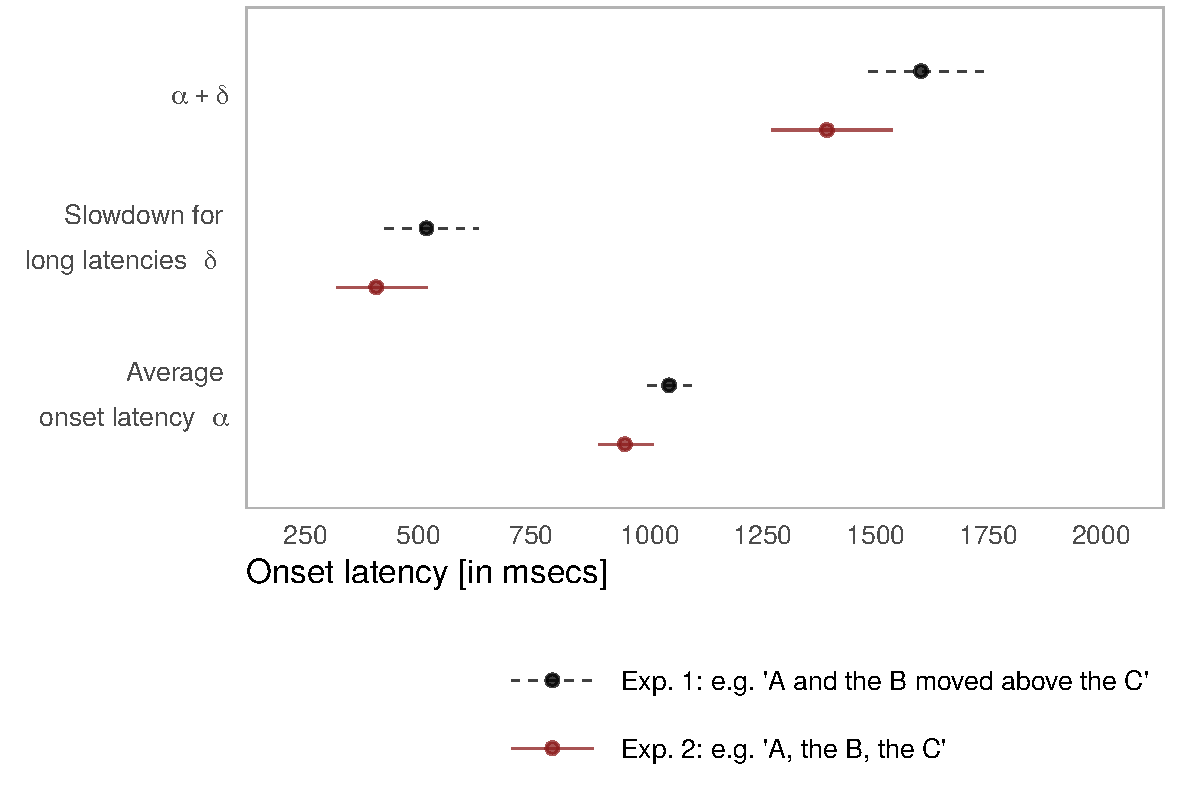
\includegraphics[scale=.5]{NPexpmoglong.pdf}
	\end{center}
\end{frame}


	\begin{frame}{Model comparisons}
\begin{scriptsize}
% latex table generated in R 4.0.2 by xtable 1.8-4 package
% Wed Aug 19 16:26:17 2020
\begin{table}[ht]
\centering
	\caption{\scriptsize{Predictive performance estimated as the \textit{expected log pointwise predictive density} ($\widehat{elpd}$). Models are ordered by predictive performance (model with highest predictive performance in top row)}. Standard error in parentheses.}
\begin{tabular}{rlrr}
  \toprule
 & Model & $\updel\widehat{elpd}$ & $\widehat{elpd}$ \\ 
  \midrule
Experiment 1 & MoG-0 & -- & -21,851 (74) \\ 
   \rowcolor{yellow!40!white}& MoG-1 & 0 (2) & -21,851 (74) \\ 
   \rowcolor{yellow!40!white}& LMM-1 & -513 (56) & -22,364 (107) \\ 
   & LMM-2 & -515 (57) & -22,366 (107) \\ 
   & LMM-0 & -519 (56) & -22,369 (107) \\ 
   \midrule
Experiment 2 & MoG-0 & -- & -14,088 (57) \\ 
   \rowcolor{yellow!40!white}& MoG-1 & -1 (1) & -14,089 (57) \\ 
   & LMM-0 & -362 (44) & -14,450 (80) \\ 
   \rowcolor{yellow!40!white}& LMM-1 & -363 (44) & -14,451 (80) \\ 
   & LMM-2 & -364 (44) & -14,452 (81) \\ 
		\bottomrule
		\end{tabular}\\
		\textit{Note.} LMM = Linear mixed effects model; MoG = Mixture of Gaussians 
		\end{table}
\end{scriptsize}
\end{frame}
	
\end{document}


